% Informe - Proyecto 1, Computacion Paralela y Distribuida (UVG)
% Compilar desde esta carpeta:  pdflatex informe.tex  (dos veces, para el indice)
% Las tablas de resultados se generan con:  python informe/generar_tablas.py

\documentclass[11pt,letterpaper]{article}

\usepackage[utf8]{inputenc}
\usepackage[T1]{fontenc}
\usepackage[spanish,es-nodecimaldot,es-noshorthands,es-tabla]{babel}
\usepackage{lmodern}
\usepackage[margin=2.5cm]{geometry}
\usepackage{graphicx}
\usepackage{booktabs}
\usepackage{longtable}
\usepackage{array}
\usepackage{float}
\usepackage{caption}
\usepackage{amsmath}
\usepackage{xcolor}
\usepackage{tikz}
\usetikzlibrary{shapes.geometric, arrows.meta, positioning}
\usepackage{pgfplots}
\pgfplotsset{compat=1.17}
\usepackage{listings}
\usepackage[hidelinks]{hyperref}

\lstset{
  basicstyle=\ttfamily\footnotesize,
  columns=fullflexible,
  keepspaces=true,
  frame=single,
  breaklines=true,
  literate={á}{{\'a}}1 {é}{{\'e}}1 {í}{{\'i}}1 {ó}{{\'o}}1 {ú}{{\'u}}1 {ñ}{{\~n}}1
}

\newcommand{\codigo}[1]{\texttt{#1}}

\begin{document}

% ---------------------------------------------------------------------------
% Caratula
% ---------------------------------------------------------------------------
\begin{titlepage}
  \centering
  {\large\bfseries UNIVERSIDAD DEL VALLE DE GUATEMALA\par}
  \vspace{0.2cm}
  {\itshape 1CC30642020261} -- Computación Paralela y Distribuida\par
  Sección 10\par
  Catedrática: Kimberly Barrera\par
  \vspace{4cm}
  {\Huge\bfseries Proyecto 1\par}
  \vspace{0.4cm}
  {\LARGE Screensaver de chuchos paralelizado con OpenMP\par}
  \vspace{4cm}
  \begin{tabular}{l}
    Isabella Obando -- 23074 \\
    Anthony Lou -- 23410 \\
    Nelson Escalante -- 22046 \\
  \end{tabular}
  \vfill
  {\large Guatemala, \today\par}
\end{titlepage}

\tableofcontents
\newpage

% ---------------------------------------------------------------------------
\section{Introducción}
% ---------------------------------------------------------------------------

Este informe documenta el diseño, la implementación y la evaluación de un
\emph{screensaver} escrito en C++ con la biblioteca gráfica SDL2 y paralelizado
con OpenMP. El programa dibuja $N$ ``chuchos'' (sprites de perros de
$64\times64$ píxeles) de colores pseudoaleatorios que se desplazan por un canvas
de $640\times480$, rebotan contra los bordes y chocan entre sí con una respuesta
basada en choques elásticos. El valor de $N$ se recibe por línea de comandos y
en pantalla se muestran los FPS junto con el tiempo que tarda la simulación.

El trabajo siguió el enfoque iterativo que propone OpenMP: primero se construyó
una versión secuencial funcional y luego se paralelizaron, una por una, las
regiones de mayor costo, verificando en cada paso que el resultado no cambiara.
Como ayuda visual, la pantalla se divide en una zona secuencial y una zona
paralela de otro color, cuyo tamaño se puede ajustar en vivo.

Además del screensaver se construyó un programa de \emph{benchmark} sin ventana
que mide la simulación para distintos valores de $N$ y de hilos, calcula el
\emph{speedup} y la eficiencia, y verifica bit a bit que la versión paralela
produzca exactamente el mismo resultado que la secuencial.

% ---------------------------------------------------------------------------
\section{Antecedentes}
% ---------------------------------------------------------------------------

\subsection{OpenMP y memoria compartida}

OpenMP es una interfaz de programación para paralelismo en memoria compartida
basada en directivas de compilador, rutinas de biblioteca y variables de
entorno~\cite{openmp52}. Su modelo de ejecución es \emph{fork--join}: un hilo
maestro crea un equipo de hilos al entrar a una región paralela y, al salir,
todos se sincronizan en una barrera implícita antes de que continúe solo el
maestro~\cite{chapman2008}. La directiva \codigo{parallel for} reparte las
iteraciones de un ciclo entre los hilos según una política de
\emph{scheduling} (\codigo{static}, \codigo{dynamic}, \codigo{guided}), y la
cláusula \codigo{if} permite decidir en tiempo de ejecución si una región se
ejecuta en paralelo o con un solo hilo\footnote{Con \codigo{if(false)} la
región se ejecuta con un equipo de un solo hilo, lo que permite usar el mismo
código para la versión secuencial y la paralela.}.

\subsection{Metodología PCAM}

Foster propone diseñar algoritmos paralelos en cuatro etapas~\cite{foster1995}:
\textbf{Partición} (descomponer el cálculo y los datos en tareas pequeñas),
\textbf{Comunicación} (identificar qué datos necesita cada tarea de las demás),
\textbf{Aglomeración} (agrupar tareas para reducir el costo de comunicación y
sincronización) y \textbf{Mapeo} (asignar los grupos a procesadores). Este
proyecto aplica PCAM a la simulación de los chuchos en la
sección~\ref{sec:pcam}.

\subsection{Speedup, eficiencia y ley de Amdahl}

Si $T_s$ es el tiempo de la mejor versión secuencial y $T_p$ el tiempo de la
versión paralela con $p$ hilos, el \emph{speedup} y la eficiencia son
\begin{equation}
  S(p) = \frac{T_s}{T_p}, \qquad E(p) = \frac{S(p)}{p}.
\end{equation}
Amdahl mostró que si una fracción $f$ del programa es inherentemente
secuencial, el speedup está acotado por~\cite{amdahl1967,pacheco2011}
\begin{equation}
  S(p) \le \frac{1}{f + \frac{1-f}{p}}.
\end{equation}
En este informe se reportan dos speedups: contra la mejor versión secuencial
($S_{\text{sec}}$) y contra la misma versión paralela con un hilo
($S_{1h}$), porque, como se verá, la versión paralela realiza el doble de
revisiones de colisión que la secuencial.

\subsection{SDL2}

SDL (\emph{Simple DirectMedia Layer}) es una biblioteca multiplataforma en C
que da acceso a ventanas, eventos de teclado y ratón, y renderizado 2D
acelerado~\cite{sdl2}. En este proyecto se usa para crear la ventana, generar
la textura del chucho a partir de un bitmap, teñirla con
\codigo{SDL\_SetTextureColorMod} y dibujar el HUD con una fuente de píxeles
propia\footnote{Se evitó depender de SDL2\_ttf para que el proyecto solo
requiera \codigo{libsdl2-dev}.}.

% ---------------------------------------------------------------------------
\section{Desarrollo}
% ---------------------------------------------------------------------------

\subsection{Descripción del screensaver}

\begin{figure}[H]
  \centering
  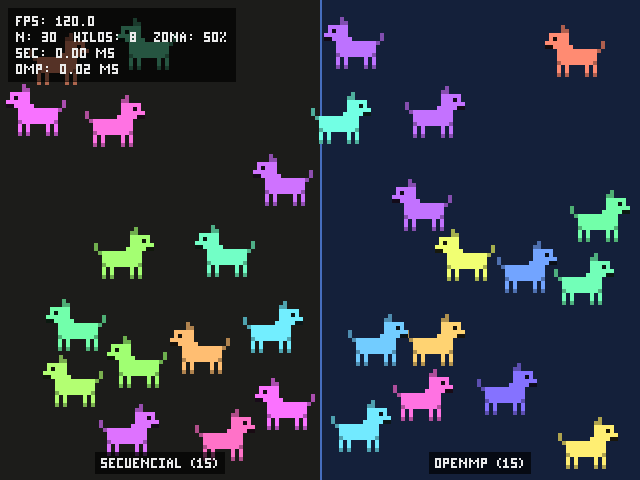
\includegraphics[width=0.7\textwidth]{figuras/zona_paralela.png}
  \caption{Screensaver con la zona paralela al 50\%: a la derecha (fondo azul)
  los chuchos se procesan con OpenMP; el HUD muestra FPS, $N$, hilos y los
  milisegundos por frame de cada zona.}
  \label{fig:zona}
\end{figure}

La Tabla~\ref{tab:requisitos} resume cómo se cumple cada requisito del
enunciado.

\begin{table}[H]
  \centering
  \caption{Requisitos del screensaver y su implementación}
  \label{tab:requisitos}
  \begin{tabular}{>{\raggedright}p{4.2cm}p{10.5cm}}
    \toprule
    Requisito & Implementación \\
    \midrule
    Parámetro $N$ & \codigo{./screensaver [N] [semilla] [-{}-zona P] [-{}-hilos H]}; todos se validan. \\
    Colores pseudoaleatorios & Tono aleatorio (HSV) por chucho con \codigo{std::mt19937}; cambia al chocar. \\
    Canvas $\geq 640\times480$ & Ventana de $640\times480$. \\
    Movimiento & Velocidad aleatoria en magnitud (60--240 px/s) y dirección. \\
    Física / trigonometría & Integración explícita, rebote en bordes, colisiones elásticas entre chuchos. \\
    Despliegue de FPS & HUD con FPS, ms por zona, $N$, hilos y tamaño de la zona. \\
    \bottomrule
  \end{tabular}
\end{table}

\subsection{Modelo físico}

Cada chucho guarda su posición $(x,y)$, velocidad $(v_x,v_y)$, tono y tinte.
En cada frame la posición se integra de forma explícita con un $\Delta t$
acotado a 0.05~s:
\begin{equation}
  x \leftarrow x + v_x\,\Delta t, \qquad y \leftarrow y + v_y\,\Delta t.
\end{equation}
Si el sprite sale del rango válido ($0 \le x \le 576$, $0 \le y \le 416$), la
posición se refleja respecto al borde y la componente de la velocidad se fuerza
a apuntar hacia adentro, lo que evita que el chucho quede ``pegado'' a la pared.

Dos chuchos $a$ y $b$ \textbf{chocan} si sus cajas envolventes
($56\times52$~px) se traslapan y además se están acercando:
\begin{equation}
  |x_a - x_b| < 56 \;\wedge\; |y_a - y_b| < 52 \;\wedge\;
  (\mathbf{p}_b - \mathbf{p}_a)\cdot(\mathbf{v}_b - \mathbf{v}_a) < 0 .
\end{equation}
La condición del producto punto evita que un par que sigue traslapado vuelva a
chocar en el frame siguiente. Si el chucho $i$ chocó con $k$ compañeros en el
frame, su nueva velocidad toma la \emph{dirección} del promedio de las
velocidades de los compañeros y la \emph{rapidez} promedio de ellos:
\begin{equation}
  \mathbf{v}_i \leftarrow \frac{\bar{\mathbf{v}}}{\lVert\bar{\mathbf{v}}\rVert}\,
  \frac{1}{k}\sum_{j}\lVert\mathbf{v}_j\rVert,
  \qquad \bar{\mathbf{v}} = \frac{1}{k}\sum_j \mathbf{v}_j .
\end{equation}
Con un solo compañero esto equivale a intercambiar velocidades (choque elástico
entre masas iguales). Se descartó promediar los vectores directamente porque en
pruebas le quitaba energía al sistema: con $N\ge100$ la rapidez promedio caía de
$\sim$150 a 0 px/s en un minuto.

\subsection{Versión secuencial}

La versión secuencial detecta colisiones recorriendo el triángulo superior de
pares ($i<j$): $N(N-1)/2$ revisiones. Cada choque se anota en un buffer (suma
de velocidades, suma de rapideces y cantidad de choques de cada chucho) y en
una segunda pasada se aplica. Separar \emph{detectar} de \emph{aplicar} hace
que el resultado no dependa del orden en que se revisan los pares.

\subsection{Diseño paralelo con PCAM}\label{sec:pcam}

\paragraph{Partición.} Se usó descomposición de dominio: la tarea mínima es
``procesar al chucho $i$'' en cada una de las tres etapas del frame (mover,
detectar choques, aplicar choques). Mover y aplicar son independientes por
chucho. Detectar es $O(N)$ por chucho y $O(N^2)$ en total, y concentra entre el 93\% y el 99\% del tiempo
(Tabla~\ref{tab:etapas}).

\paragraph{Comunicación.} Para detectar, la tarea $i$ necesita leer la
posición y velocidad de todos los demás chuchos (comunicación global de solo
lectura). En la versión de triángulo, un choque entre $i$ y $j$ escribe en las
entradas $i$ \emph{y} $j$ del buffer; en paralelo, dos hilos podrían escribir
la misma entrada $j$ al mismo tiempo (condición de carrera).

\paragraph{Aglomeración.} Para eliminar la condición de carrera sin
\emph{locks} ni operaciones atómicas, cada tarea $i$ recorre la fila completa
($j=0,\dots,N-1$, $j\neq i$), acumula en variables locales y escribe
únicamente su propia entrada del buffer. El costo es duplicar las revisiones
($N(N-1)$ en lugar de $N(N-1)/2$). Como cada chucho suma a sus compañeros en el
mismo orden que en la versión de triángulo, el resultado es idéntico bit a bit.

\paragraph{Mapeo.} Las iteraciones se reparten con
\codigo{schedule(static)}: al recorrer la fila completa todas cuestan lo mismo,
así que bloques contiguos e iguales balancean la carga sin costo de
coordinación. El número de hilos se toma de \codigo{-{}-hilos} o del valor por
defecto de OpenMP (8 en el equipo de pruebas).

\subsection{Secciones paralelas y sincronización}

Las tres etapas usan la misma directiva, con la cláusula \codigo{if} para
decidir si corren en paralelo:
\begin{lstlisting}[language=C++]
#pragma omp parallel for schedule(static) if (paralelo)
for (int k = 0; k < m; ++k) {
    const int i = indices[k];   // cada hilo escribe solo en sus propios i
    ...
}
\end{lstlisting}
Los mecanismos de sincronización y protección de memoria compartida son:
\begin{itemize}
  \item \textbf{Barreras implícitas} al final de cada \codigo{parallel for}:
  garantizan que todos los chuchos se movieron antes de detectar, y que todos
  terminaron de detectar antes de aplicar (aplicar modifica las velocidades que
  detectar lee).
  \item \textbf{Propiedad exclusiva de datos}: en cada etapa el hilo que procesa
  al chucho $i$ es el único que escribe su estado y su entrada del buffer; las
  lecturas a los demás chuchos ocurren en una etapa donde nadie los modifica.
  \item \textbf{Acumuladores locales} (privados de cada hilo) durante la
  detección, escritos al buffer compartido una sola vez al final.
\end{itemize}
Los buffers se reservan una vez y se reutilizan entre frames
(\codigo{std::vector}); SDL se inicializa y se destruye en orden inverso, y
cada error de inicialización libera lo ya creado antes de salir.

\subsection{Zona paralela visual}

Para visualizar la paralelización, al inicio de cada frame los chuchos se
clasifican según la posición de su centro: los que están en la franja derecha
(la zona paralela, de fondo azul) se procesan con OpenMP y el resto con un solo
hilo. El porcentaje de la zona se elige con \codigo{-{}-zona P} (0 = todo
secuencial, 100 = todo paralelo) o en vivo con las flechas, y el HUD muestra
cuánto tarda cada zona por frame (Figura~\ref{fig:zona}).

\subsection{Metodología de medición}

Las mediciones se hicieron con el programa \codigo{build/benchmark}, que corre
la simulación \emph{sin ventana} para que el dibujo no contamine los tiempos:
\begin{itemize}
  \item Equipo: Intel Core i5-1035G1 (4 núcleos físicos, 8 hilos lógicos),
  Ubuntu 24.04 en WSL2, g++ 13.3 con \codigo{-O2 -fopenmp}.
  \item $N \in \{500, 1000, 2000, 4000\}$ y hilos $\in \{1, 2, 4, 8\}$.
  \item Por prueba: 10 repeticiones; cada una recrea la escena con la semilla
  7, corre 5 frames de calentamiento y mide 30 frames con $\Delta t$ fijo de
  $1/60$~s. Se reporta el promedio de ms por frame.
  \item Al terminar, el estado final de cada corrida paralela se compara bit a
  bit con el de la secuencial.
\end{itemize}
El FPS del screensaver real se midió aparte, con 8 segundos por corrida y
\codigo{OMP\_WAIT\_POLICY=passive} (ver sección~\ref{sec:discusion}).

% ---------------------------------------------------------------------------
\section{Resultados}
% ---------------------------------------------------------------------------

\begin{table}[H]
  \centering
  \caption{Tiempo de simulación por frame, speedup contra la mejor versión
  secuencial ($S$ sec), contra OpenMP con un hilo ($S$ 1h) y eficiencia $E$.}
  \label{tab:resumen}
  \small
  \begin{tabular}{rlrrrrrr}
\toprule
$N$ & Versión & Hilos & ms/frame & Desv. & $S$ (sec) & $S$ (1h) & $E$ \\
\midrule
500 & secuencial & -- & 0.503 & 0.019 & 1.00 & -- & 1.00 \\
500 & openmp & 1 & 1.031 & 0.059 & 0.49 & 1.00 & 0.49 \\
500 & openmp & 2 & 0.542 & 0.059 & 0.93 & 1.90 & 0.46 \\
500 & openmp & 4 & 0.335 & 0.053 & 1.50 & 3.08 & 0.37 \\
500 & openmp & 8 & 0.253 & 0.082 & 1.99 & 4.08 & 0.25 \\
\midrule
1000 & secuencial & -- & 1.926 & 0.052 & 1.00 & -- & 1.00 \\
1000 & openmp & 1 & 3.780 & 0.102 & 0.51 & 1.00 & 0.51 \\
1000 & openmp & 2 & 2.064 & 0.184 & 0.93 & 1.83 & 0.47 \\
1000 & openmp & 4 & 1.501 & 0.102 & 1.28 & 2.52 & 0.32 \\
1000 & openmp & 8 & 1.064 & 0.239 & 1.81 & 3.55 & 0.23 \\
\midrule
2000 & secuencial & -- & 8.216 & 0.429 & 1.00 & -- & 1.00 \\
2000 & openmp & 1 & 16.472 & 0.913 & 0.50 & 1.00 & 0.50 \\
2000 & openmp & 2 & 9.025 & 0.316 & 0.91 & 1.83 & 0.46 \\
2000 & openmp & 4 & 6.167 & 0.149 & 1.33 & 2.67 & 0.33 \\
2000 & openmp & 8 & 4.724 & 1.075 & 1.74 & 3.49 & 0.22 \\
\midrule
4000 & secuencial & -- & 36.187 & 1.995 & 1.00 & -- & 1.00 \\
4000 & openmp & 1 & 73.634 & 9.150 & 0.49 & 1.00 & 0.49 \\
4000 & openmp & 2 & 46.585 & 8.269 & 0.78 & 1.58 & 0.39 \\
4000 & openmp & 4 & 33.432 & 2.381 & 1.08 & 2.20 & 0.27 \\
4000 & openmp & 8 & 27.433 & 3.326 & 1.32 & 2.68 & 0.16 \\
\bottomrule
\end{tabular}

\end{table}

\begin{figure}[H]
  \centering
  \begin{tikzpicture}
    \begin{axis}[
      width=0.75\textwidth, height=6.5cm,
      xlabel={Hilos}, ylabel={Speedup vs. secuencial},
      xtick={1,2,4,8}, xmode=log, log basis x=2,
      log ticks with fixed point,
      ymin=0, grid=major, legend pos=north west,
    ]
      \addplot+[mark=*] coordinates {(1,0.488) (2,0.928) (4,1.500) (8,1.988)};
\addlegendentry{$N=500$}
\addplot+[mark=*] coordinates {(1,0.509) (2,0.933) (4,1.284) (8,1.810)};
\addlegendentry{$N=1000$}
\addplot+[mark=*] coordinates {(1,0.499) (2,0.910) (4,1.332) (8,1.739)};
\addlegendentry{$N=2000$}
\addplot+[mark=*] coordinates {(1,0.491) (2,0.777) (4,1.082) (8,1.319)};
\addlegendentry{$N=4000$}

      \addplot[dashed, gray, domain=1:8, samples=2] {x};
      \addlegendentry{Ideal}
    \end{axis}
  \end{tikzpicture}
  \caption{Speedup de la versión OpenMP respecto a la mejor versión secuencial.}
  \label{fig:speedup}
\end{figure}

\begin{table}[H]
  \centering
  \caption{Tiempo por etapa (ms por frame): secuencial y OpenMP con 8 hilos.}
  \label{tab:etapas}
  \small
  \begin{tabular}{rlrrrr}
\toprule
$N$ & Versión & Mover (ms) & Detectar (ms) & Aplicar (ms) & \% detectar \\
\midrule
500 & Secuencial & 0.003 & 0.468 & 0.032 & 93.0\% \\
500 & OpenMP 8h & 0.008 & 0.204 & 0.040 & 80.8\% \\
1000 & Secuencial & 0.006 & 1.856 & 0.064 & 96.3\% \\
1000 & OpenMP 8h & 0.046 & 0.910 & 0.108 & 85.5\% \\
2000 & Secuencial & 0.012 & 8.075 & 0.129 & 98.3\% \\
2000 & OpenMP 8h & 0.164 & 4.246 & 0.314 & 89.9\% \\
4000 & Secuencial & 0.029 & 35.867 & 0.291 & 99.1\% \\
4000 & OpenMP 8h & 0.766 & 25.537 & 1.130 & 93.1\% \\
\bottomrule
\end{tabular}

\end{table}

\begin{table}[H]
  \centering
  \caption{FPS del screensaver real (incluye dibujar) con 8 hilos. En el
  screensaver, la zona 0\% usa el mismo recorrido completo que OpenMP pero con
  un solo hilo, por eso sus ms de simulación son mayores que los de la versión
  secuencial del benchmark.}
  \label{tab:fps}
  \small
  \begin{tabular}{rrrrrr}
\toprule
& \multicolumn{2}{c}{Secuencial (zona 0\%)} & \multicolumn{2}{c}{OpenMP (zona 100\%)} & \\
\cmidrule(lr){2-3}\cmidrule(lr){4-5}
$N$ & FPS & ms sim. & FPS & ms sim. & Mejora FPS \\
\midrule
250 & 246.0 & 0.40 & 160.1 & 1.50 & 0.65$\times$ \\
500 & 94.0 & 2.60 & 96.0 & 2.08 & 1.02$\times$ \\
1000 & 46.1 & 9.13 & 51.7 & 3.90 & 1.12$\times$ \\
2000 & 18.6 & 34.68 & 22.5 & 12.27 & 1.21$\times$ \\
\bottomrule
\end{tabular}

\end{table}

En todas las pruebas el estado final de la versión paralela fue idéntico bit a
bit al de la secuencial (columna \codigo{resultado\_identico} del CSV).

\subsection{Discusión}\label{sec:discusion}

\begin{itemize}
  \item \textbf{La detección de colisiones domina.} Entre el 93\% y el 99\% del tiempo del
  frame está en la etapa $O(N^2)$ (Tabla~\ref{tab:etapas}); mover y aplicar son
  $O(N)$ y casi despreciables. Por eso paralelizar solo el movimiento, como se
  pensó al inicio, no habría dado ganancia visible.
  \item \textbf{Costo de eliminar la condición de carrera.} La versión OpenMP
  con un hilo tarda cerca del doble que la secuencial ($S_{\text{sec}}\approx
  0.5$), porque revisa cada par dos veces. Por eso el speedup contra 1 hilo
  ($S_{1h}$) es alto, pero el speedup real contra la mejor versión secuencial
  queda en aproximadamente la mitad.
  \item \textbf{Hardware.} El equipo tiene 4 núcleos físicos; pasar de 4 a 8
  hilos usa \emph{hyper-threading}, que comparte las unidades de cómputo de
  cada núcleo, por lo que la ganancia de 4 a 8 hilos es menor y la eficiencia
  cae.
  \item \textbf{Temperatura.} En una laptop la frecuencia baja tras carga
  sostenida; en una corrida previa, $N=4000$ (que se mide al final) salió
  hasta 35\% más lento que al medirlo solo con el equipo frío. Por eso se
  reporta el promedio de 10 repeticiones y la desviación estándar.
  \item \textbf{Política de espera de OpenMP.} En el screensaver el dibujo
  también corre en CPU (llvmpipe en WSLg). Con la espera activa por defecto,
  los hilos de OpenMP que ``giran'' tras cada región le roban núcleos al
  render y los FPS paralelos llegaron a ser menores que los secuenciales; con
  \codigo{OMP\_WAIT\_POLICY=passive} la versión paralela sí mejora los FPS. En
  el benchmark sin ventana ocurre lo contrario: \codigo{passive} empeora el
  tiempo porque despertar a los hilos en cada región cuesta de 0.1 a 0.4~ms.
  \item \textbf{FPS.} Los FPS del screensaver dependen también del dibujo, que
  es secuencial; por la ley de Amdahl la mejora en FPS es menor que la mejora
  en el tiempo de simulación. Con $N$ pequeño ($N=250$) la versión paralela
  incluso da menos FPS (Tabla~\ref{tab:fps}): la simulación tarda menos de
  0.5~ms y el costo de crear y sincronizar el equipo de hilos en cada región
  supera la ganancia. La paralelización conviene a partir de
  $N\approx500$.
\end{itemize}

% ---------------------------------------------------------------------------
\section{Conclusiones}
% ---------------------------------------------------------------------------

\begin{enumerate}
  \item Se implementó un screensaver en C++/SDL2 que cumple los requisitos del
  enunciado, con una versión secuencial y una paralela con OpenMP que se
  pueden comparar en vivo mediante la zona paralela.
  \item La región con mayor potencial de paralelización es la detección de
  colisiones ($O(N^2)$), que concentra entre el 93\% y el 99\% del tiempo de
  simulación.
  \item Reorganizar la detección para que cada hilo escriba solo sus propios
  datos eliminó las condiciones de carrera sin \emph{locks} ni atómicos, y
  produce resultados idénticos bit a bit a la versión secuencial, a costa de
  duplicar el número de revisiones.
  \item El speedup real contra la mejor versión secuencial está limitado por
  ese trabajo extra, por los 4 núcleos físicos del equipo y por el
  \emph{throttling} térmico; el speedup contra la versión paralela con un hilo
  muestra buena escalabilidad hasta 4 hilos.
  \item En una aplicación gráfica, la política de espera de los hilos de
  OpenMP puede importar tanto como el algoritmo: la espera activa compite con
  el renderizado por software.
\end{enumerate}

\section{Recomendaciones}

\begin{itemize}
  \item Implementar una versión paralela que conserve el triángulo $i<j$
  usando un buffer privado por hilo y una reducción final, con
  \codigo{schedule(dynamic)} o \codigo{guided} por el desbalance del
  triángulo, y compararla contra la versión actual.
  \item Reducir la complejidad de la detección con una rejilla espacial
  (\emph{uniform grid}), de modo que cada chucho solo revise a sus vecinos.
  \item Medir en un equipo con GPU para que el dibujo no compita por la CPU
  con los hilos de OpenMP.
\end{itemize}

% ---------------------------------------------------------------------------
\begin{thebibliography}{9}
\bibitem{amdahl1967}
G.~M. Amdahl, ``Validity of the single processor approach to achieving large
scale computing capabilities,'' en \emph{Proc. AFIPS Spring Joint Computer
Conference}, 1967, pp.~483--485.

\bibitem{chapman2008}
B.~Chapman, G.~Jost y R.~van~der~Pas, \emph{Using OpenMP: Portable Shared
Memory Parallel Programming}. Cambridge, MA: MIT Press, 2008.

\bibitem{foster1995}
I.~Foster, \emph{Designing and Building Parallel Programs}. Reading, MA:
Addison-Wesley, 1995.

\bibitem{openmp52}
OpenMP Architecture Review Board, \emph{OpenMP Application Programming
Interface, Version 5.2}, 2021. [En línea]. Disponible:
\url{https://www.openmp.org/specifications/}

\bibitem{pacheco2011}
P.~Pacheco, \emph{An Introduction to Parallel Programming}. Burlington, MA:
Morgan Kaufmann, 2011.

\bibitem{sdl2}
SDL Project, \emph{Simple DirectMedia Layer 2 -- Documentation Wiki}. [En
línea]. Disponible: \url{https://wiki.libsdl.org/SDL2/}
\end{thebibliography}

% ---------------------------------------------------------------------------
\newpage
\appendix
\section{Anexo 1 -- Diagrama de flujo del programa}
% ---------------------------------------------------------------------------

El programa no pide datos de forma interactiva durante la ejecución: los
parámetros se leen de la línea de comandos y, durante la animación, el usuario
puede ajustar la zona paralela con las flechas o salir con Esc o cerrando la
ventana. Los bloques azules son secciones paralelas; cada una termina en una
barrera implícita.

\begin{figure}[H]
\centering
\scriptsize
\begin{tikzpicture}[
  node distance=0.28cm,
  >={Stealth[length=2mm]},
  base/.style={draw, align=center, minimum width=5.2cm, minimum height=0.6cm},
  term/.style={base, ellipse, minimum width=2.6cm, fill=gray!15},
  proc/.style={base, rectangle, rounded corners=2pt},
  io/.style={base, trapezium, trapezium left angle=75, trapezium right angle=105, fill=yellow!15},
  dec/.style={draw, diamond, aspect=3.2, align=center, inner sep=0pt, fill=orange!15},
  par/.style={proc, fill=blue!15},
  err/.style={proc, minimum width=3.6cm, fill=red!10},
]
  \node[term] (inicio) {Inicio};
  \node[io, below=of inicio] (args) {Captura de argumentos:\\ $N$, semilla, \texttt{-{}-zona P}, \texttt{-{}-hilos H}};
  \node[dec, below=of args] (valido) {¿Argumentos\\ válidos?};
  \node[proc, below=of valido] (hilos) {Si se indicó, \texttt{omp\_set\_num\_threads(H)}};
  \node[proc, below=of hilos] (sdl) {Inicializar SDL, ventana, renderer\\ y textura del chucho};
  \node[dec, below=of sdl] (sdlok) {¿Todo se\\ creó bien?};
  \node[proc, below=of sdlok] (crear) {\texttt{crearChuchos(N, semilla)}: posición,\\ velocidad y tono aleatorios};
  \node[io, below=of crear] (eventos) {Leer eventos: flechas ajustan la zona};
  \node[dec, below=of eventos] (salir) {¿Esc o cerrar\\ ventana?};
  \node[proc, below=of salir] (clasif) {Clasificar chuchos por zona\\ (secuencial / paralela)};
  \node[par, below=of clasif] (mover) {Mover y rebotar\\ \texttt{parallel for} + barrera};
  \node[par, below=of mover] (detectar) {Detectar choques (fila completa)\\ \texttt{parallel for} + barrera};
  \node[par, below=of detectar] (aplicar) {Aplicar choques\\ \texttt{parallel for} + barrera};
  \node[io, below=of aplicar] (dibujar) {Despliegue: fondo, chuchos, etiquetas\\ y HUD (FPS, ms por zona)};

  \node[err, right=1.2cm of valido] (uso) {Imprimir uso\\ y salir (código 1)};
  \node[err, right=1.2cm of sdlok] (errsdl) {Mostrar error, liberar\\ lo creado, salir (1)};
  \node[io, right=1.2cm of salir, minimum width=3.6cm] (fin1) {Imprimir FPS y ms\\ promedio};
  \node[proc, below=0.4cm of fin1, minimum width=3.6cm] (fin2) {Destruir textura,\\ renderer y ventana};
  \node[term, below=0.4cm of fin2] (fin) {Fin};

  \draw[->] (inicio) -- (args);
  \draw[->] (args) -- (valido);
  \draw[->] (valido) -- node[right] {sí} (hilos);
  \draw[->] (valido) -- node[above] {no} (uso);
  \draw[->] (hilos) -- (sdl);
  \draw[->] (sdl) -- (sdlok);
  \draw[->] (sdlok) -- node[right] {sí} (crear);
  \draw[->] (sdlok) -- node[above] {no} (errsdl);
  \draw[->] (crear) -- (eventos);
  \draw[->] (eventos) -- (salir);
  \draw[->] (salir) -- node[right] {no} (clasif);
  \draw[->] (salir) -- node[above] {sí} (fin1);
  \draw[->] (fin1) -- (fin2);
  \draw[->] (fin2) -- (fin);
  \draw[->] (clasif) -- (mover);
  \draw[->] (mover) -- (detectar);
  \draw[->] (detectar) -- (aplicar);
  \draw[->] (aplicar) -- (dibujar);
  \draw[->] (dibujar.west) -- ++(-0.8,0) |- (eventos.west);
\end{tikzpicture}
\caption{Diagrama de flujo del screensaver. En la zona secuencial las mismas
etapas azules corren con un solo hilo (\texttt{if(false)}).}
\end{figure}

El benchmark sigue el mismo esquema sin ventana: valida sus argumentos
(\codigo{-{}-n}, \codigo{-{}-hilos}, \codigo{-{}-frames}, \codigo{-{}-reps},
\codigo{-{}-semilla}, \codigo{-{}-salida}), y para cada $N$ y cantidad de hilos
repite la simulación, mide cada etapa con \codigo{omp\_get\_wtime()}, verifica
el estado final contra el secuencial y escribe la tabla en consola y los CSV.

% ---------------------------------------------------------------------------
\newpage
\section{Anexo 2 -- Catálogo de funciones}
% ---------------------------------------------------------------------------

\footnotesize
\setlength{\tabcolsep}{4pt}
\begin{longtable}{>{\raggedright}p{3.5cm}>{\raggedright}p{3.7cm}>{\raggedright}p{2.7cm}p{5.0cm}}
\toprule
Función / clase & Entradas & Salidas & Descripción \\
\midrule
\endhead
\multicolumn{4}{l}{\textbf{\texttt{src/main.cpp}}} \\
\texttt{main} & \texttt{int argc, char* argv[]}: argumentos del programa & \texttt{int}: código de salida & Valida argumentos, inicializa SDL, crea la simulación y corre el ciclo eventos $\to$ simulación $\to$ dibujo; al salir imprime promedios y libera recursos. \\
\texttt{parsearArgumentos} & \texttt{argc, argv}; \texttt{Opciones\& op} & \texttt{bool}: argumentos válidos; llena \texttt{op} (n, semilla, zona, hilos) & Lee $N$ y semilla posicionales y las opciones \texttt{-{}-zona} (0--100) y \texttt{-{}-hilos} (1--1024). \\
\texttt{procesarEventos} & \texttt{ZonaParalela\& zona} & \texttt{bool}: seguir ejecutando & Atiende cerrar ventana y Esc; las flechas cambian el tamaño de la zona. \\
\midrule
\multicolumn{4}{l}{\textbf{\texttt{src/argumentos.cpp}}} \\
\texttt{parsearEntero} & \texttt{const char* texto}; \texttt{long min, max} & \texttt{bool}; \texttt{long\& salida} & Convierte texto a entero con \texttt{strtol}, rechazando texto extra, desbordes y valores fuera de rango. \\
\texttt{parsearLista\allowbreak Enteros} & \texttt{const char* texto} (ej. \texttt{"1,2,4"}); \texttt{min, max} & \texttt{bool}; \texttt{vector<int>\& salida} & Separa por comas y valida cada elemento con \texttt{parsearEntero}. \\
\midrule
\multicolumn{4}{l}{\textbf{\texttt{src/chucho.cpp}, \texttt{src/color.cpp}}} \\
\texttt{struct Chucho} & -- & -- & Estado de un chucho: \texttt{x, y, vx, vy} (float), \texttt{tono}, \texttt{tinte} (RGB) y \texttt{pausaColor}. \\
\texttt{crearChuchos} & \texttt{int n}; \texttt{unsigned semilla} & \texttt{vector<Chucho>} & Crea $n$ chuchos con posición, velocidad (60--240 px/s, ángulo aleatorio) y tono pseudoaleatorios (\texttt{mt19937}). \\
\texttt{colorDesdeTono} & \texttt{float tono} (grados) & \texttt{Color} (RGB) & Normaliza el tono a $[0,360)$ y lo convierte con \texttt{hsvARgb} usando la saturación y brillo de \texttt{config.h}. \\
\texttt{hsvARgb} & \texttt{float h, s, v} & \texttt{Color} & Conversión estándar de HSV a RGB. \\
\midrule
\multicolumn{4}{l}{\textbf{\texttt{src/zona.cpp}}} \\
\texttt{ZonaParalela} & \texttt{int porcentaje} & objeto & Franja derecha de la pantalla procesada con OpenMP. \\
\texttt{ajustar} & \texttt{int delta} & -- & Suma \texttt{delta} al porcentaje, acotado a $[0,100]$. \\
\texttt{inicioX} & -- & \texttt{int}: píxel donde empieza la zona & $640 - 640\cdot p/100$. \\
\texttt{contiene} & \texttt{const Chucho\& c} & \texttt{bool} & Verdadero si el centro del chucho está en la zona. \\
\midrule
\multicolumn{4}{l}{\textbf{\texttt{src/simulacion.cpp}}} \\
\texttt{moverChuchos} & \texttt{vector<Chucho>\&}; \texttt{const vector<int>\& indices}; \texttt{float dt}; \texttt{bool paralelo} & chuchos modificados & Integra la posición, rebota en bordes y descuenta la pausa de color. \textbf{Sección paralela} (\texttt{parallel for static if(paralelo)}). \\
\texttt{rebotarEje} & \texttt{float\& pos, float\& vel}; \texttt{min, max} & \texttt{pos}, \texttt{vel} corregidos & Refleja la posición en el borde y fuerza la velocidad hacia adentro. \\
\texttt{medirMs} & función \texttt{f} & \texttt{double}: ms & Ejecuta \texttt{f} y mide su duración con \texttt{omp\_get\_wtime}. \\
\texttt{Simulacion::\allowbreak paso} & \texttt{float dt}; \texttt{const ZonaParalela\&} & \texttt{TiemposFrame} (ms secuencial y paralelo) & Clasifica por zona y ejecuta mover, detectar y aplicar para cada zona, midiendo cada una. \\
\texttt{Simulacion::\allowbreak clasificar} & \texttt{const ZonaParalela\&} & listas de índices por zona & Separa los chuchos según la zona de su centro. \\
\midrule
\multicolumn{4}{l}{\textbf{\texttt{src/colisiones.cpp} (\texttt{ManejadorColisiones})}} \\
\texttt{preparar} & \texttt{int n} & buffers de tamaño $n$ & Ajusta el tamaño de los buffers (se reutilizan entre frames). \\
\texttt{detectar} & \texttt{const vector<Chucho>\&}; \texttt{indices}; \texttt{bool paralelo} & buffers \texttt{sumaVx\_}, \texttt{sumaVy\_}, \texttt{sumaRapidez\_}, \texttt{choques\_} & Cada chucho revisa a todos los demás y escribe solo su entrada del buffer, usando acumuladores locales. \textbf{Sección paralela}, sin condiciones de carrera. \\
\texttt{detectarTriangulo} & \texttt{const vector<Chucho>\&} & mismos buffers & Versión secuencial de referencia: recorre solo $i<j$ y escribe en $i$ y $j$. Resultado idéntico a \texttt{detectar}. \\
\texttt{aplicar} & \texttt{vector<Chucho>\&}; \texttt{indices}; \texttt{bool paralelo} & chuchos con nueva velocidad y tono & Aplica dirección y rapidez promedio de los compañeros; gira el tono si pasó la pausa. \textbf{Sección paralela}. \\
\texttt{seTraslapan} & \texttt{const Chucho\& a, b} & \texttt{bool} & Prueba de cajas envolventes de $56\times52$. \\
\texttt{seAcercan} & \texttt{const Chucho\& a, b} & \texttt{bool} & Producto punto de posición y velocidad relativas negativo. \\
\midrule
\multicolumn{4}{l}{\textbf{\texttt{src/estadisticas.cpp}, \texttt{src/hud.cpp}, \texttt{src/render.cpp}, \texttt{src/texto.cpp}, \texttt{src/sprite.cpp}}} \\
\texttt{Estadisticas::\allowbreak registrarFrame} & \texttt{float dt}; \texttt{const TiemposFrame\&} & valores actuales y totales & Acumula FPS y ms por zona; recalcula los valores del HUD cada 0.5~s. \\
\texttt{fpsPromedio}, \texttt{tiemposPromedio} & -- & \texttt{float}, \texttt{TiemposFrame} & Promedios de toda la corrida, impresos al salir. \\
\texttt{crearTexturaChucho} & \texttt{SDL\_Renderer*} & \texttt{SDL\_Texture*} (o \texttt{nullptr}) & Genera la textura de $64\times64$ a partir de un bitmap de $16\times16$ escalado 4 veces. \\
\texttt{dibujarFondo} & \texttt{SDL\_Renderer*}; \texttt{const ZonaParalela\&} & -- & Pinta la zona secuencial, la zona paralela (azul) y la línea divisoria. \\
\texttt{dibujarChuchos} & \texttt{SDL\_Renderer*}; \texttt{SDL\_Texture*}; \texttt{const vector<Chucho>\&} & -- & Dibuja cada chucho con su tinte, volteado según su dirección. \\
\texttt{dibujarEtiquetas\allowbreak Zonas} & renderer; zona; \texttt{int} chuchos por zona & -- & Escribe ``SECUENCIAL ($n$)'' y ``OPENMP ($n$)'' al pie de cada zona. \\
\texttt{dibujarHud} & \texttt{SDL\_Renderer*}; \texttt{const DatosHud\&} & -- & Recuadro con FPS, $N$, hilos, zona y ms por zona. \\
\texttt{dibujarTexto}, \texttt{anchoTexto}, \texttt{altoTexto} & texto; posición; escala & -- / \texttt{int} & Fuente de píxeles propia (A--Z, 0--9 y símbolos). \\
\midrule
\multicolumn{4}{l}{\textbf{\texttt{bench/} (programa de benchmark)}} \\
\texttt{medir} & \texttt{const ConfigMedicion\&} ($n$, versión, hilos, frames, calentamiento, repeticiones, semilla) & \texttt{Resultado\allowbreak Medicion} & Corre la simulación sin ventana y mide ms por frame de cada etapa en cada repetición. \\
\texttt{pasoMedido} & chuchos; índices; colisiones; versión & \texttt{TiemposEtapas\&} acumulado & Un frame con dt fijo, midiendo mover, detectar y aplicar. \\
\texttt{mismosEstados} & dos \texttt{vector<Chucho>} & \texttt{bool} & Compara campo por campo, bit a bit. \\
\texttt{armarReporte} & \texttt{vector<Resultado\allowbreak Medicion>} & \texttt{vector<Fila\allowbreak Reporte>} & Calcula speedup (vs.\ secuencial y vs.\ 1 hilo), eficiencia y verificación. \\
\texttt{imprimirTabla}, \texttt{escribirCsv}, \texttt{escribirCsvDetalle} & filas; ruta & consola / archivos CSV & Despliegue de resultados. \\
\bottomrule
\end{longtable}
\normalsize

% ---------------------------------------------------------------------------
\newpage
\section{Anexo 3 -- Bitácora de pruebas}
% ---------------------------------------------------------------------------

Cada prueba es una combinación de $N$ y versión, con 10 mediciones (M1--M10).
Cada medición es el promedio de ms por frame de 30 frames. $S$ es el speedup
contra la versión secuencial y $E$ la eficiencia ($S/p$).

\begin{table}[H]
\centering\small
\caption{Bitácora de mediciones, $N=500$ (ms por frame de simulación)}
\begin{tabular}{lrrrrr}
\toprule
Medición & Secuencial & OMP 1h & OMP 2h & OMP 4h & OMP 8h \\
\midrule
M1 & 0.531 & 0.958 & 0.593 & 0.337 & 0.179 \\
M2 & 0.521 & 0.977 & 0.509 & 0.354 & 0.224 \\
M3 & 0.511 & 0.969 & 0.504 & 0.344 & 0.248 \\
M4 & 0.510 & 1.002 & 0.516 & 0.252 & 0.185 \\
M5 & 0.514 & 1.018 & 0.513 & 0.316 & 0.272 \\
M6 & 0.473 & 1.014 & 0.575 & 0.348 & 0.189 \\
M7 & 0.489 & 1.116 & 0.683 & 0.347 & 0.293 \\
M8 & 0.501 & 1.108 & 0.516 & 0.457 & 0.196 \\
M9 & 0.474 & 1.049 & 0.509 & 0.299 & 0.449 \\
M10 & 0.504 & 1.102 & 0.499 & 0.301 & 0.294 \\
\midrule
Promedio & 0.503 & 1.031 & 0.542 & 0.335 & 0.253 \\
Desv. estándar & 0.019 & 0.059 & 0.059 & 0.053 & 0.082 \\
Speedup $S$ & 1.000 & 0.488 & 0.928 & 1.500 & 1.988 \\
Eficiencia $E$ & 1.000 & 0.488 & 0.464 & 0.375 & 0.248 \\
\bottomrule
\end{tabular}
\end{table}

\begin{table}[H]
\centering\small
\caption{Bitácora de mediciones, $N=1000$ (ms por frame de simulación)}
\begin{tabular}{lrrrrr}
\toprule
Medición & Secuencial & OMP 1h & OMP 2h & OMP 4h & OMP 8h \\
\midrule
M1 & 2.012 & 3.851 & 1.906 & 1.413 & 0.985 \\
M2 & 1.980 & 3.785 & 1.984 & 1.498 & 1.719 \\
M3 & 1.950 & 3.912 & 2.149 & 1.510 & 1.114 \\
M4 & 1.856 & 3.965 & 1.978 & 1.498 & 1.082 \\
M5 & 1.868 & 3.687 & 1.972 & 1.530 & 0.971 \\
M6 & 1.899 & 3.730 & 1.974 & 1.734 & 0.996 \\
M7 & 1.919 & 3.791 & 1.976 & 1.503 & 0.941 \\
M8 & 1.873 & 3.693 & 1.993 & 1.329 & 0.994 \\
M9 & 1.968 & 3.652 & 2.181 & 1.476 & 0.909 \\
M10 & 1.935 & 3.736 & 2.527 & 1.518 & 0.928 \\
\midrule
Promedio & 1.926 & 3.780 & 2.064 & 1.501 & 1.064 \\
Desv. estándar & 0.052 & 0.102 & 0.184 & 0.102 & 0.239 \\
Speedup $S$ & 1.000 & 0.509 & 0.933 & 1.284 & 1.810 \\
Eficiencia $E$ & 1.000 & 0.509 & 0.467 & 0.321 & 0.226 \\
\bottomrule
\end{tabular}
\end{table}

\begin{table}[H]
\centering\small
\caption{Bitácora de mediciones, $N=2000$ (ms por frame de simulación)}
\begin{tabular}{lrrrrr}
\toprule
Medición & Secuencial & OMP 1h & OMP 2h & OMP 4h & OMP 8h \\
\midrule
M1 & 8.192 & 16.629 & 9.388 & 6.111 & 7.384 \\
M2 & 7.982 & 16.114 & 8.793 & 6.139 & 4.091 \\
M3 & 8.152 & 18.948 & 9.281 & 6.364 & 4.059 \\
M4 & 8.205 & 16.619 & 8.506 & 6.081 & 4.034 \\
M5 & 7.915 & 15.961 & 8.902 & 6.166 & 4.875 \\
M6 & 9.379 & 16.012 & 9.115 & 6.222 & 4.042 \\
M7 & 7.861 & 16.495 & 8.605 & 6.439 & 4.126 \\
M8 & 8.065 & 15.946 & 9.275 & 5.953 & 5.681 \\
M9 & 8.178 & 16.018 & 9.365 & 6.186 & 4.717 \\
M10 & 8.227 & 15.979 & 9.024 & 6.006 & 4.235 \\
\midrule
Promedio & 8.216 & 16.472 & 9.025 & 6.167 & 4.724 \\
Desv. estándar & 0.429 & 0.913 & 0.316 & 0.149 & 1.075 \\
Speedup $S$ & 1.000 & 0.499 & 0.910 & 1.332 & 1.739 \\
Eficiencia $E$ & 1.000 & 0.499 & 0.455 & 0.333 & 0.217 \\
\bottomrule
\end{tabular}
\end{table}

\begin{table}[H]
\centering\small
\caption{Bitácora de mediciones, $N=4000$ (ms por frame de simulación)}
\begin{tabular}{lrrrrr}
\toprule
Medición & Secuencial & OMP 1h & OMP 2h & OMP 4h & OMP 8h \\
\midrule
M1 & 34.522 & 73.285 & 38.507 & 32.071 & 25.752 \\
M2 & 34.324 & 73.992 & 41.193 & 33.453 & 26.268 \\
M3 & 34.959 & 72.982 & 39.310 & 33.519 & 27.013 \\
M4 & 34.832 & 98.165 & 40.834 & 31.850 & 35.185 \\
M5 & 40.255 & 67.041 & 44.904 & 35.607 & 22.660 \\
M6 & 37.835 & 68.132 & 46.083 & 32.748 & 25.451 \\
M7 & 38.166 & 75.656 & 60.025 & 30.676 & 26.774 \\
M8 & 35.551 & 71.247 & 62.433 & 30.534 & 29.899 \\
M9 & 34.662 & 68.979 & 46.428 & 37.620 & 26.723 \\
M10 & 36.764 & 66.862 & 46.136 & 36.247 & 28.608 \\
\midrule
Promedio & 36.187 & 73.634 & 46.585 & 33.432 & 27.433 \\
Desv. estándar & 1.995 & 9.150 & 8.269 & 2.381 & 3.326 \\
Speedup $S$ & 1.000 & 0.491 & 0.777 & 1.082 & 1.319 \\
Eficiencia $E$ & 1.000 & 0.491 & 0.388 & 0.271 & 0.165 \\
\bottomrule
\end{tabular}
\end{table}


\subsection*{Captura de las mediciones}

Salida en consola de \codigo{make bench}:

\lstinputlisting[basicstyle=\ttfamily\tiny,breaklines=false]{../resultados/benchmark_consola.txt}

\begin{figure}[H]
  \centering
  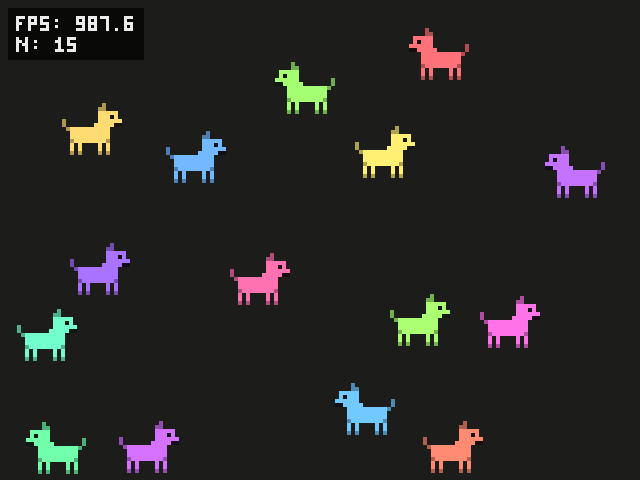
\includegraphics[width=0.6\textwidth]{figuras/chuchos.png}
  \caption{Screensaver tras 10 segundos de simulación con choques.}
\end{figure}

% ---------------------------------------------------------------------------
\section{Material suplementario}
% ---------------------------------------------------------------------------

\begin{itemize}
  \item Repositorio: \url{https://github.com/anthonylouschwank/Proyecto-Paralela}
  \item Compilación y ejecución (Ubuntu/WSL, requiere \codigo{libsdl2-dev}):
\begin{lstlisting}
make                                   # screensaver y benchmark
make run N=2000 ARGS="7 --zona 100"    # screensaver
make bench                             # benchmark -> resultados/*.csv
python informe/generar_tablas.py       # tablas de este informe
\end{lstlisting}
\end{itemize}

\end{document}
